\documentclass[11pt,a4paper]{article}
\usepackage[a4paper,margin=2cm]{geometry}
\usepackage[]{graphicx}
\usepackage{bm}
\usepackage{apacite}
\bibliographystyle{apacite}
\usepackage{svg}
\usepackage{multirow}
\usepackage{amsmath}
\setlength{\parindent}{0pt}
\usepackage{pgf}
\usepackage{tikz}
\usepackage{pgfplots}
\usepackage{wrapfig}
\usepackage{float}
\usepackage[autostyle, english = american]{csquotes}
\usepackage[toc,page]{appendix}
\usepackage{amssymb}
\MakeOuterQuote{"}
\usepackage[T1]{fontenc}
\usepackage{enumitem}

\renewcommand{\baselinestretch}{1.1}
\setlist[enumerate]{itemsep=0mm}
\setlist[itemize]{itemsep=-0.7mm}
\begin{document}
	\nocite{*}
	
	\begin{titlepage}
		
		
		\title{Determining the effect of electrolyte concentration of the voltage produced by galvanic cells}
		
		\author{Noah Alexiou}
		
		
		\date{June 2025}
		
		\maketitle
		\centering
		
	\end{titlepage}
	\tableofcontents
	\newpage
	
	
	\section{Rationale}
	
	
	\subsection{Background}

	

	\textbf{Redox}
	
	Redox reactions are reactions that involve the transfer of electrons between atoms. These reactions commonly occur within galvanic cells, which within themselves contain two half cells. 
	

	\textbf{Half Cells}
	
	Half cells consists of an electrolyte solution and electrode. When two are connected through a load and a salt  bridge, one of these half cells will become the anode, where oxidation occurs, and the other will become the cathode, where reduction occurs. The oxidised cell will transfer its electrons across a wire, where they will then reach and be accepted by the reduced cell.
	
	Each cell has its own standard electrode potential ($E^0$) which dictates the magnitude of electron emission, or attraction it has under standard lab conditions. 
	
	By measuring the difference in magnitude between cells, the overall potential between the cells can be quantified. 
	
	$$
	E^0_{\textrm{ Cell}}=E^0_{\textrm{ Cathode}}-E^0_{\textrm{ Anode}}
	$$
	
	For this experiment, the half cells will be made up of zinc and copper, which have $E^0$ values of $-0.7618$V, and $+0.3419$V respectively. Cell's with this composition are also known as "Daniel Cell's", and will have a theoretical voltage, under standard conditions, of: $$(0.3419-(-0.7618))=1.1037\textrm{V}$$
	
	

	\textbf{The Nernst Equation}\newline
	The Nernst equation is a mathematical equation that allows the theoretical voltage potential of a cell to be quantified under non-standard conditions. While factors such as temperature and pressure throughout the experiment were not modified, the reaction quotient $(Q)$ was indirectly altered by the change in $[CuSO_4]$. 
\newline The Nernst equation can be defined as:
	$$
	E_{\textrm{cell}}=E^0 - \frac{RT}{nF}\cdot \ln(Q)
	$$
	Where:
	\begin{itemize}
		\item $E$ = Theoretical electrode potential (voltage)of the cell
		\item $E^0$ = Standard electrode potential of the cell
		\item $T$ = Temperature in kelvin 
		\item $R$ = Universal gas constant
		\item $F$= Faraday constant
		\item $z$ = Number of moles of electrons transferred
		\item $Q$ = Reaction Quotient
		

	\end{itemize}
Substituting 
\begin{align*}
E_{\textrm{cell}}=(0.3419+0.7618)-\frac{8.31446261815324\cdot298}{2\cdot96485}&\cdot\ln\frac{[Zn^{2+}]}{[Cu^{2+}]}\\
E_{\textrm{cell}}=(0.3419+0.7618)-\frac{8.31446261815324\cdot298}{2\cdot96485}&\cdot\ln\frac{1}{[Cu^{2+}]} \because [Zn^{2+}]\textrm{ remains constant}
\end{align*}

\begin{figure}

	\centering

	\begin{tikzpicture}
		\begin{axis}[xmin=0, xmax=2, ymin=1.03, xlabel=${ \left[Cu^{2+}\right] }$, ylabel=$E_{\textrm{cell}}$, width=0.8\paperwidth, height=6cm]
			\addplot
		[
		samples=2000, smooth
		]
		{
				(0.3419+0.7618)-((8.31446261815324*298)/(2*96485))*ln(x^(-1))
		};
		\end{axis}
		
	\end{tikzpicture}
 
		\caption{The theoretical relationship between $E_{\textrm{cell}}$ and $[Cu^{2+}]$}
		\label{ogLog}
\end{figure}
\newpage
Considering figure \ref{ogLog}, the theoretical change in $E_\textrm{cell}$ is minuscule in comparison to the change in $[Cu^{2+}]$. The when the $x$-axis increases from 0.5 to 1, a change of only $0.009$V is observed. If the relationship is further considered, with domain [0.5, 2], increasing concentration by a factor of 4 only results in an an additional $0.018$V. It was questioned whether this relationship held true, especially as $\lim\limits_{x\to 0}$.

Investigation of $[Cu^{2+}]=[0, 1]$ would theoretically be the most distinguishable from a logarithmic relationship if it differs due to the distinct curve observed in the area. 

Clearly $[Zn^{2+}]=[Cu^{2+}]\neq 0$, as this would either result in a division by 0, or $\ln(0)$, which are both undefined. 
\subsection{Research Question}
How does altering $[CuSO_4]$ at low concentrations (0-1 mol) affect its voltage output, and does the observed relationship follow the theoretical relationship when applying the Nernst equation.
\section{Methodology}
\subsection{Modifications}

The following modifications were made to the original experiment. The original method can be found in the appendix section.\newline
\textbf{Half Cell Compositions}\newline
The results of original experiment indicated that copper and aluminium produced the largest voltage. It was theorised that after multiple trials, the aluminium would oxidise, skewing results.

It was decided that copper and zinc would be more suitable as although they produced a smaller voltage, zinc would take longer to oxidise and therefore producer more consistent results.

\textbf{Electrodes}\newline
Rather than thin strips, larger plates were bent into a "C" shape, slightly smaller than the diameter of the beaker they would be placed in. This maximised the surface area in contact with the electrolyte solution. Furthermore by reusing the same electrodes, this surface area was constant for all trials.

\textbf{Measurement devices}\newline
A digital multimeter was substituted in place of the conventional analog volt meter. Since the digital multimeter uses digital logic to measure voltage, rather than a magnetic field induced by the flow of current, the digital multimeter should reduce the ions 'used up' during each measurement. Furthermore the digital output measures volts to 3 decimal places, leading to reduced uncertainty and increased precision. 

\textbf{Salt Bridge}\newline
The salt bridge was unaltered, and still made from filter paper, however, care was taken to ensure consistency in their size.

\textbf{Procedure}\newline
The electrolyte solutions were pre-mixed, labelled, and stored in sealed containers prior to the start of the experiment. This reduced the potential for errors in procedure, as well as the time it took to conduct the experiment, which reduced the influence of environmental factors, such as changes in temperature, on results.

\subsection{Method}
\textbf{Materials}
\begin{itemize}
	\item 30ml $CuSO_4$ at concentrations $1.00\textrm{M}, 0.85\textrm{M}, 0.70\textrm{M}, 0.55\textrm{M}, 0.40\textrm{M}, 0.30\textrm{M}, 0.20\textrm{M}, 0.10\textrm{M}$
	\item 240ml $1$M$\;ZnSO_4$
	\item 20ml $KNO_3$
	\item Petri dish
	\item $50\textrm{ml}$ Beaker - x$2$
	\item Zinc sheet $\approx4\textrm{cm}\times6\textrm{cm}$ 
	\item Copper sheet $\approx4\textrm{cm}\times6\textrm{cm}$ 
	\item Emery paper
	\item Filter paper strips $\approx 2\textrm{cm}\times10\textrm{cm}$
	\item Digital Multimeter
	\item Alligator clips
	\item 150ml Plastic bottle - x16
	\item Tweezers 
	\item 1L Distilled water
	\item Emery paper
\end{itemize}
\newpage
\textbf{Procedure}
\small
\begin{enumerate}
	\item Pour varying amounts of $CUSO_4$ into 150ml plastic bottles and dilute with distilled water to form solutions with concentrations $1.00\textrm{M}, 0.85\textrm{M}, 0.70\textrm{M}, 0.55\textrm{M}, 0.40\textrm{M}, 0.30\textrm{M}, 0.20\textrm{M and } 0.10\textrm{M}$.
	
	\item Fill 8 of the 150ml plastic bottles with 30ml of 1M $ZnSO_4$ and set aside with copper solutions. 
	
	\item Polish electrodes with emery paper until they their entire surface is free of visible oxidation then connect to alligator clips.
	
	\item Connect alligator clips to multimeter and set to DC voltage mode.
	
	\item Transfer the contents of a $CUSO_4$, and $ZnSO_4$ container into separate beakers.
	
	\item Wet salt bridge with $KNO_3$ and rest over the lip of both beakers, so that it is partially submerged in both. 
	
	\item Add the electrodes to the solution and record result as soon as value settles.
	
	\item Remove electrodes immediately and wash with distilled water. Stir electrolyte solutions with a glass stir rod. Remove salt bridge and dispose of.
	
	\item Reconstruct cell with a new salt bridge, add electrodes back, and repeat measurementation so that there are three trials in total for any given concentration.
	
	\item Safely dispose of electrolyte solutions, wash equipment, and repeat for next $CUSO_4$ concentration.
\end{enumerate}

\subsection{Risk assessment}
\tiny
\begin{tabular}{|p{3cm}|p{4cm}|p{4.5cm}|p{4cm}|}

	\hline
	\textbf{Item/Substance} & \textbf{Potential Hazards} & \textbf{Standard Handling Procedures} & \textbf{Disposal} \\
	\hline
	Alligator clip with lead & Clip may cause pain and injury if applied to skin. & & \\
	\hline
	Glass beaker & Breakage of beaker. Cuts from chipped rims. & Inspect and discard any chipped or cracked beakers. Sweep up broken glass with brush and dustpan; do not use fingers. & \\
	\hline
	Metal tweezers & Can be used as a weapon if long and sharply pointed. & & \\
	\hline
	Disposable plastic gloves & May easily be punctured, allowing entry of liquid. Latex gloves may cause an allergic reaction to some people& Take care not to puncture. Check for punctures before use. Use a type of glove that is suitable for the chemicals to be used. & \\
	\hline
	Lab coat & \textbf{Flammable}. Sleeves may catch on objects and knock them over. & & \\
	\hline
	Safety glasses & Scratched or dirty glasses may hinder vision, causing headaches during prolonged use. & \textbf{Each person should preferably have own safety glasses}. Check and, if necessary, clean glasses before each use.. & \\
	\hline
	Filter paper & \textbf{Flammable}. \textbf{Used filter paper may contain harmful residues}. & After use, dispose of residue and filter paper appropriately. & Dispose of residue and filter paper appropriately. \\
	\hline
	Aluminum (pieces) & Not toxic. \textbf{Sharp points and edges may cause injury to skin and eyes}. & & \textbf{May be placed in the garbage}. \\
	\hline
	Copper (sheet) & Not toxic. & & $<$1 kg/day may be placed in the garbage. Larger quantities should be retained for collection by a waste service or metal recycler. \\
	\hline
	Copper(II) sulfate ($>$0.94 M) & \textbf{Toxic}. \textbf{Irritates skin and eyes}. & $<$5 mL/day may be poured down the drain. Larger quantities should be placed in a Copper waste container. &\\
	\hline
	Iron (nails) & Not toxic. Usually mild steel. Sharp edges and points may cause injury. & Store in a dry location to prevent rusting of iron surfaces. & \textbf{May be placed in the garbage}. \\
	\hline


	Iron(III) chloride ($>$0.93 M) (ferric chloride) & \textbf{CORROSIVE TO SKIN, EYES AND LUNGS}. May be corrosive to metals. \textbf{Harmful if swallowed}. Causes skin irritation. \textbf{Causes serious eye damage}. & Solubility $\sim$550 g/L at 20$^\circ$C. Undergoes hydrolysis at low concentrations with precipitation of iron(III) hydroxide. & $<$200 mL/day may be poured into 10 times the volume of water and poured down the drain in a stream of water. \\
	\hline
		Zinc (pieces) & Not toxic to humans. & & \textbf{May be placed in the garbage}. \\
	\hline
	Zinc nitrate (0.79-1 M) & \textbf{Toxic}. \textbf{Irritates skin, eyes and lungs}. \textbf{Harmful if swallowed}. Causes skin irritation. \textbf{Causes serious eye irritation}. \textbf{Very toxic to aquatic life with long lasting effects}. & & $<$5 mL/day may be diluted with 10 times the volume of water and poured down the drain. Larger quantities should be placed in a Zinc waste container. \\
	\hline
	Potassium nitrate (0.1-1 M) & \textbf{May irritate eyes and skin}. GHS data: Not classified as a hazardous chemical. & & $<$1 L/day may be poured down the drain in a stream of water. \\
	\hline
	Aluminum nitrate ($>$0.5 M) & \textbf{Irritates skin and eyes, due to acidity} as a result of reaction with water. \textbf{Causes mild skin irritation}. & & $<$100 mL/day may be added slowly with stirring to 20 times the mass of water, then poured down the drain in a stream of water. \\
	\hline
	Spatula & Properties depend on spatula material. A nickel spatula may cause an allergic skin reaction, especially if used repeatedly. & People with nickel allergy should wear gloves if using a nickel spatula. & \\
	\hline
	Wash bottle & May be used to spray others. & Preferably use distilled water. Change water regularly to avoid microbial growth. & \\
	\hline
\end{tabular}
\newpage
\normalsize

\section{Results}
\begin{figure}[h]
	\centering
\begin{tabular}{|c|c|c|c|c|c|}
	\hline
	[$CuSO_4$] & \multicolumn{3}{|c|}{Voltage}   & Mean & sigma \\
	\hline
	& Trial 1 & Trial 2 & Trial 3 &  &  \\
	\hline
	1 & 0.703 & 0.678 & 0.661 & 0.681 & 0.021 \\
	\hline
	0.85 & 0.664 & 0.623 & 0.488 & 0.592 & 0.088 \\
	\hline
	0.7 & 0.557 & 0.455 & 0.472 & 0.495 & 0.051 \\
	\hline
	0.55 & 0.457 & 0.422 & 0.413 & 0.431 & 0.022 \\
	\hline
	0.4 & 0.438 & 0.412 & 0.416 & 0.422 & 0.013 \\
	\hline
	0.3 & 0.498 & 0.47 & 0.476 & 0.481 & 0.014 \\
	\hline
	0.2 & 0.458 & 0.487 &  {\color{red}0.399} & 0.4725 & 0.0145 \\
	\hline
	0.1 & 0.405 & 0.456 & 0.463 & 0.441 & 0.029 \\
	\hline
\end{tabular}
\caption{Raw data with calculations. Outliers (highlighted in {\color{red} red}) \textbf{not} included in calculations}
\end{figure}
\begin{figure}[h]
	\centering
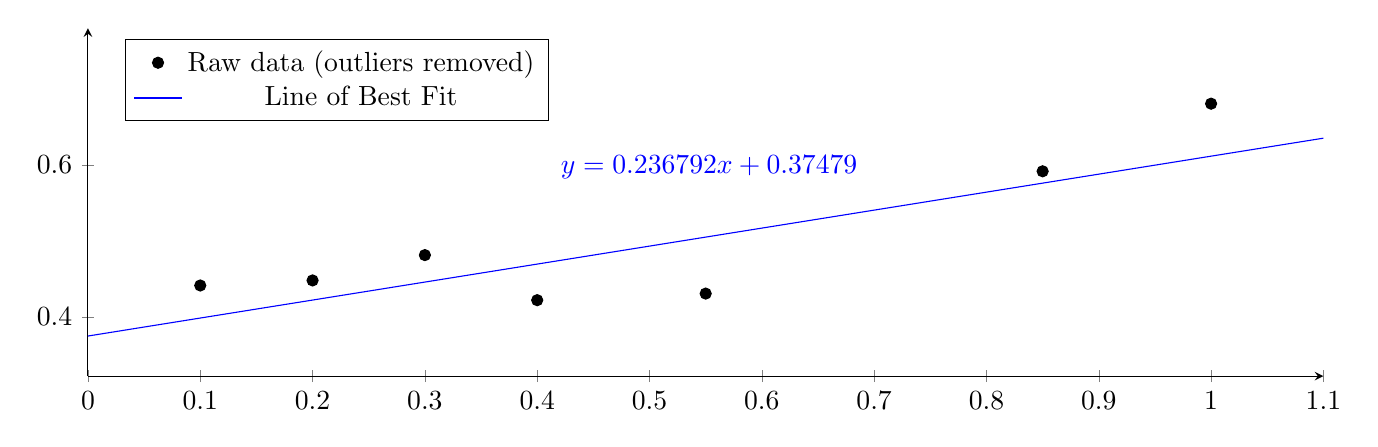
\begin{tikzpicture}
	\begin{axis}[xmin=0, xmax=1.1, ymin=0.322, ymax=0.78, axis lines=left, scale mode=stretch to fill, width=0.8\paperwidth, height=6cm, xtick distance=0.1, ytick distance=0.2, legend pos=north west]
		\addplot[only marks, mark=*, color=black]
		coordinates {
			(1, 0.680666666666667)
			(0.85, 0.591666666666667)
			(0.55, 0.430666666666667)
			(0.4, 0.422)
			(0.3, 0.481333333333333)
			(0.2, 0.448)
			(0.1, 0.441333333333333)
		};
		\addplot[no markers, blue, domain=0:1.1, samples=2, xlabel=] {(0.236792*x) + 0.37479};
	\node [anchor=south west,inner ysep=2.5cm, inner xsep=6cm, color=blue] {$y=0.236792x+0.37479$};
	\legend{Raw data (outliers removed), Line of Best Fit}
	\end{axis}
\end{tikzpicture}
\caption{Raw results (outliers removed) with linear line of best fit.}
\end{figure}

\begin{figure}[h]
	\centering
	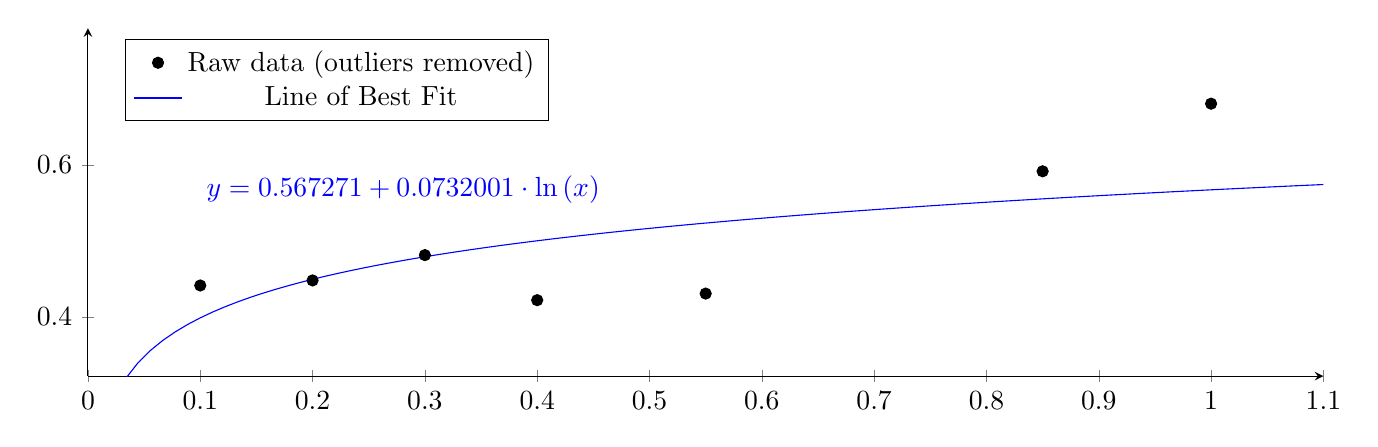
\begin{tikzpicture}
		\begin{axis}[xmin=0, xmax=1.1, ymin=0.322, ymax=0.78, axis lines=left, scale mode=stretch to fill, width=0.8\paperwidth, height=6cm, xtick distance=0.1, ytick distance=0.2, legend pos=north west]
			\addplot[only marks, mark=*, color=black]
			coordinates {
				(1, 0.680666666666667)
				(0.85, 0.591666666666667)
				(0.55, 0.430666666666667)
				(0.4, 0.422)
				(0.3, 0.481333333333333)
				(0.2, 0.448)
				(0.1, 0.441333333333333)
			};
			\addplot[no markers, blue, domain=0:1.1, samples=100, xlabel=] {0.567271+0.0732001*ln(x)};
			\node [anchor=south west,inner ysep=3cm, inner xsep=1.5cm, color=blue] {$y=0.567271+0.0732001\cdot\ln\left(x\right)$};
			\legend{Raw data (outliers removed), Line of Best Fit}
		\end{axis}
	\end{tikzpicture}
	\caption{Raw results (outliers removed) with logarithmic line of best fit.}
\end{figure}


\subsection{Analysis of Evidence}
The scatter plot produced using experimental data suggests a linear relationship. Using desmos, a linear regression can be utilised to find the line of best fit. 





Theory would suggest it should be logarithmic 

if we substitute the parameters of the nirnst equation (this part needs more working)

consider half equation $Cu^{2+}+Zn \rightarrow Zn^{2+} + Cu$ \textbf{(possibly show how half equation is derived)}

finding Q: Since Cu2+ and Zn2+ are the only aqueous parts of each side of the half equation, they're the only ones counted
there's a linear relationship

\begin{align*}
	(0.3419+0.7618)-&\frac{8.31446261815324\cdot298}{2\cdot96485}\cdot\ln\frac{[Zn^{2+}]}{[Cu^{2+}]}\\
	\\
	(0.3419+0.7618)-&\frac{8.31446261815324\cdot298}{2\cdot96485}\cdot\ln\frac{1}{1}\\
	&=1.1037\textrm{V}
\end{align*}


GRAPH COMPARING THEM

another trend observed was lowering voltage over trials 




\begin{figure}[h]

	\centering
\begin{tikzpicture}
	\centering
	\begin{axis}[xmax=3.1, xmin=0.9, ymax=0.8, ymin=0.3, width=0.82\paperwidth, scale mode=stretch to fill, height=8cm, axis lines=box, clip=false, legend style={font=\small}, legend style={at={(0.3, 0.94)}},  xtick distance=1, xlabel={Trial Number}]
		
		\addplot [only marks, color=cyan,mark options={opacity=0.3}]
		coordinates{
		(1, 0.703)
		(1, 0.664)
		(1, 0.557)
		(1, 0.457)
		(1, 0.438)
		(1, 0.498)
		(1, 0.458)
		(1, 0.405)
	};

		\addplot [only marks, color=black, mark options={opacity=0.3}]
		coordinates{
		(2, 0.678)
		(2, 0.623)
		(2, 0.455)
		(2, 0.422)
		(2, 0.412)
		(2, 0.47)
		(2, 0.487)
		(2, 0.456)
	};

		\addplot [only marks, color=blue, mark options={opacity=0.3}]
		coordinates{
		(3, 0.661)
		(3, 0.488)
		(3, 0.472)
		(3, 0.413)
		(3, 0.416)
		(3, 0.476)
		(3, 0.463)		
		};
		
		
		 \addplot [,
		only marks, color=red
		] 
		coordinates {
		(1, 0.5225)
		(2, 0.500375)
		(3, 0.484142857)		
};

	    \addplot [
		error bars,
		y dir=both,y explicit
		] coordinates {
		(1, 0.5225) +- (0.149, 0.149)
		(2, 0.500375) +- (0.133, 0.133)
		(3, 0.484142857) +- (0.124, 0.124)		};



		\node[anchor=south west, inner ysep=4cm, inner xsep=8.7cm]{$y=-0.0192471x+0.540788$};
		\node[anchor=south west, inner ysep=3.5cm, inner 	xsep=8.7cm]{$R^2=0.9922$};
			
	
		

		
		\legend{Trial 1 Results, Trial 2 Results, Trial 3 Results, Average,LR of Average};
	\end{axis}
\end{tikzpicture}
\caption{Line of best fit for average voltage over sequential trials (outliers removed)}
\label{lowingVoltage}
\end{figure}

Figure \ref{lowingVoltage} depicts a trend observed where as trials continued, the voltage of each subsequent trial decreased slightly. Procedure was considered and it was theorized that this was due to reuse of the same electrolyte solution over multiple trials. The number of ions left on solution likely decreased as measurements were taken and depending on the duration of each trial and measurement phase, which is theorized to have resulted in lower voltage. While the change in voltage is only on average $-0.02$V per trial, considering $R^2=0.9922$, the linear regression has a very high correlation with the average.

\section{Discussion}

\subsection{Improvements}
Sources of error/improvements

\begin{itemize}
	\item Alligator clips in solution (floating voltage)
	\item Inconsistent measurement time. (outlier is main case of this).
	\item Alligator clips sitting in electrolyte during experiment.
	\item Temperature and pressure unknown on day of experimentation. This means that the nerenst equation cannot account for them. Therefore difference in between nernst equation and actual results n
\end{itemize}
\end{document}